\documentclass{scrartcl}

\usepackage{listings}
\usepackage{graphicx}
\usepackage{amsmath}

\title{Design of Embedded System\\Exercise 8}
\author{Erin van der Veen - s4431200\\
	Brigel Pineti - s1005549}

\begin{document}
\maketitle

\section*{8a}
\begin{figure}[!h]
	\centering
	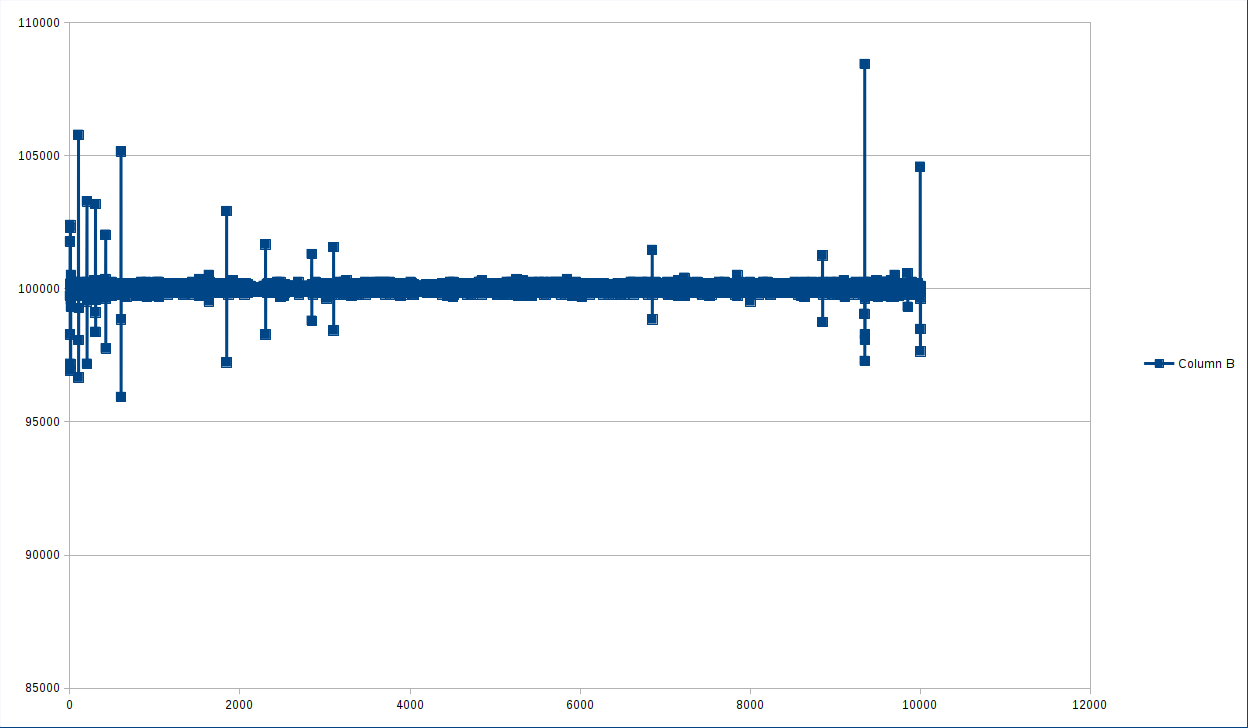
\includegraphics[width=0.8\textwidth]{resulta}
	\caption{Result of Experiment 08a}
	\label{figure:8a}
\end{figure}

See Figure~\ref{figure:8a} for the results of the experiment.
When parsing the data, we calculate an average of 99999.4639288569, very close to the desired average of 100000.
We can also conclude that 64\% of the other results fall within a 197.385072108175 of the average.
In general, there are only a few extreme outliers.
Most notably the peak at T=5284, which has many periods near it that are reasonably far below 100000.

The extreme that lays furthest below the desired period is T=7185.
It can be noted that the deviation of the upper extreme is much higher than the deviation of the lower extreme.
In fact, this can be said to be true in the general case.

\section*{8b}
\begin{figure}[!h]
	\centering
	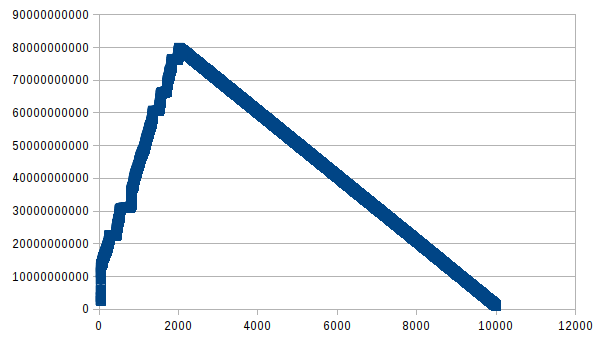
\includegraphics[width=0.8\textwidth]{resultb}
	\caption{Result of Experiment 08b}
	\label{figure:8b}
\end{figure}

See Figure~\ref{figure:8a} for the results of the experiment.
Unfortunately, due to various issues, we were unable to obtain any useful data in this experiment.
The average ``delay'' was: 41491975733.5959, with a standard deviation of: 22284406173.8658.

\end{document}
